\documentclass[]{article}
\usepackage[a4paper, total={15cm,23cm}]{geometry}
\usepackage{fancyhdr}
\usepackage{graphicx}
\usepackage{amsmath}
\usepackage{amssymb}
\usepackage{xcolor}
\usepackage{tikz}
\usepackage{verbatim}
\usepackage{tcolorbox}
\usepackage{textcomp}
\usepackage{xcomment}
\usepackage{xstring}
\usepackage{array}
%opening
\title{Visual Vector Addition}
\author{Benjamin Bauml}
\date{Spring 2024}
\pagestyle{fancy}
\rhead{PH 221}
\chead{Spring 2024}
\lhead{Week 1}

% Version 2024-02-21
% Changes
% 2024-02-21 Added xstring package to enable smooth implementation of new \ModePage command.
% For Assignment, leave Purpose as 1. For Worksheet, set to 2. For Student Solution, set to 3. For Teacher Solution, set to 4.
\newcommand{\Purpose}{4}

\newcommand{\Exclusion}{0}
\newcommand{\PageTurn}{0}
\newcommand{\GrayProb}{0}
\newcommand{\Tipsy}{0}

% Assignment
\if\Purpose1
\renewcommand{\Exclusion}{1}
\fi
% Worksheet
\if\Purpose2
\renewcommand{\Exclusion}{1}
\renewcommand{\PageTurn}{1}
\fi
% Student Solution
\if\Purpose3
\renewcommand{\PageTurn}{1}
\renewcommand{\GrayProb}{1}
\fi
% Teaching Copy
\if\Purpose4
\renewcommand{\PageTurn}{1}
\renewcommand{\GrayProb}{1}
\renewcommand{\Tipsy}{1}
\fi

\if\Exclusion1
\xcomment{Title,Problem,ProblemSub,PassFig}
\fi

\def \NewQ {0}
\def \PForce {0}
\newcommand{\MaybePage}[1]{
	\def \PForce {#1}
	\if\PForce1
		\newpage
	\else
		\if\NewQ0
		\gdef \NewQ {\PageTurn}
		\else
		\newpage
		\fi
	\fi
}

\newcommand{\ModePage}[1]{
	\IfSubStr{#1}{\Purpose}{\newpage}{}
}

\newenvironment{Problem}[2][0]{%The first argument is optional, and if it is set to 1, the \newpage will be forced.
\MaybePage{#1}
\section*{#2}
\if\GrayProb1
\begin{tcolorbox}[colback=lightgray,colframe=lightgray,sharp corners,boxsep=1pt,left=0pt,right=0pt,top=0pt,bottom=0pt,after skip=2pt]
\else
\begin{tcolorbox}[colback=white,colframe=white,sharp corners,boxsep=1pt,left=0pt,right=0pt,top=0pt,bottom=0pt,after skip=2pt]
\fi
}{
\end{tcolorbox}\noindent
}

\newenvironment{ProblemSub}[1][0]{%The argument is optional, and if a string of numbers is entered into it, it will force a \newpage in any \Purpose that shows up in the string. For example, "13" would lead to the newpage being forced in modes 1 and 3.
\ModePage{#1}
\if\GrayProb1
\begin{tcolorbox}[colback=lightgray,colframe=lightgray,sharp corners,boxsep=1pt,left=0pt,right=0pt,top=0pt,bottom=0pt,after skip=2pt]
\else
\begin{tcolorbox}[colback=white,colframe=white,sharp corners,boxsep=1pt,left=0pt,right=0pt,top=0pt,bottom=0pt,after skip=2pt]
\fi
}{
\end{tcolorbox}\noindent
}

\newenvironment{PassFig}{\begin{figure}[h]}{\end{figure}}

\newcommand{\TeachingTips}[1]{
\if\Tipsy1
\begin{tcolorbox}[colback=lightgray,colframe=black]
#1
\end{tcolorbox}
\fi
}

\newenvironment{Title}{\maketitle}{}

\begin{document}
\begin{Title}
\begin{center}
	This material is borrowed/adapted from PH 201 Tutorial 1 for Fall 2020.
\end{center}
\end{Title}

\begin{Problem}{Activity}
	Add or subtract the following vectors.
\end{Problem}
In the solutions below, the first vector is colored {\color{blue}blue}, the second vector {\color{red}red}, and the resultant vector {\color{purple}purple}. Where applicable, both the ``tail-to-tip'' and the ``parallelogram'' method were used.

\begin{PassFig}
	\centering
	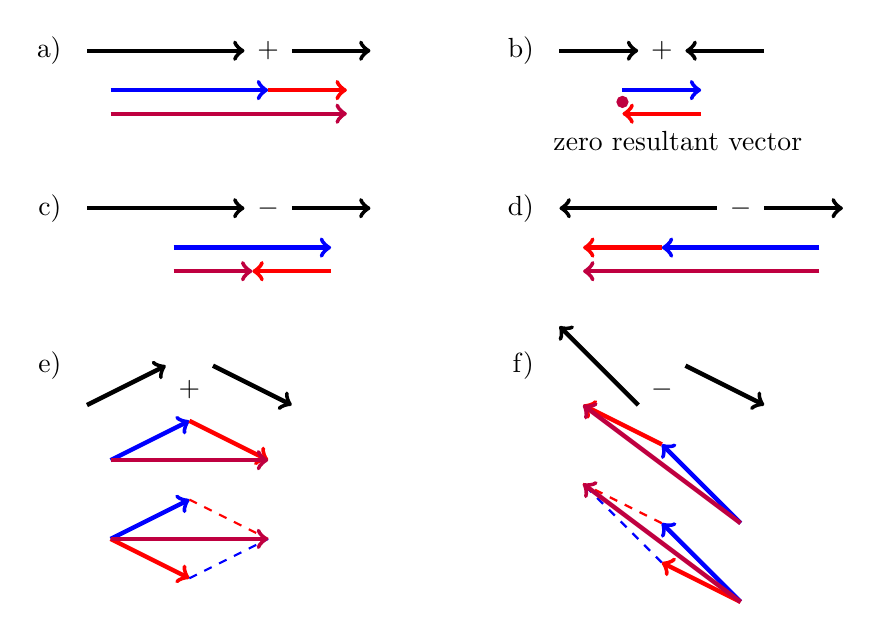
\begin{tikzpicture}
		\begin{scope}[shift={(0,0)}]
			\node[anchor=east] at (0,0) {a)};
			\draw[->,ultra thick,shift={(0.2,0)}] (0,0) -- (2,0);
			\node at (2.5,0) {$+$};
			\draw[->,ultra thick,shift={(2.8,0)}] (0,0) -- (1,0);
			\if\GrayProb1
			\draw[->,blue,ultra thick,shift={(0.5,-0.5)}] (0,0) -- (2,0);
			\draw[->,red,ultra thick,shift={(2.5,-0.5)}] (0,0) -- (1,0);
			\draw[->,purple,ultra thick,shift={(0.5,-0.8)}] (0,0) -- (3,0);
			\fi
		\end{scope}
		\begin{scope}[shift={(6,0)}]
			\node[anchor=east] at (0,0) {b)};
			\draw[->,ultra thick,shift={(0.2,0)}] (0,0) -- (1,0);
			\node at (1.5,0) {$+$};
			\draw[->,ultra thick,shift={(1.8,0)}] (1,0) -- (0,0);
			\if\GrayProb1
			\draw[->,blue,ultra thick,shift={(1,-0.5)}] (0,0) -- (1,0);
			\draw[->,red,ultra thick,shift={(1,-0.8)}] (1,0) -- (0,0);
			\filldraw[purple] (1,-0.65) circle (2pt);
			\node[anchor=north west] at (0,-0.9) {zero resultant vector};
			\fi
		\end{scope}
		\begin{scope}[shift={(0,-2)}]
			\node[anchor=east] at (0,0) {c)};
			\draw[->,ultra thick,shift={(0.2,0)}] (0,0) -- (2,0);
			\node at (2.5,0) {$-$};
			\draw[->,ultra thick,shift={(2.8,0)}] (0,0) -- (1,0);
			\if\GrayProb1
			\draw[->,blue,ultra thick,shift={(1.3,-0.5)}] (0,0) -- (2,0);
			\draw[->,red,ultra thick,shift={(2.3,-0.8)}] (1,0) -- (0,0);
			\draw[->,purple,ultra thick,shift={(1.3,-0.8)}] (0,0) -- (1,0);
			\fi
		\end{scope}
		\begin{scope}[shift={(6,-2)}]
			\node[anchor=east] at (0,0) {d)};
			\draw[->,ultra thick,shift={(0.2,0)}] (2,0) -- (0,0);
			\node at (2.5,0) {$-$};
			\draw[->,ultra thick,shift={(2.8,0)}] (0,0) -- (1,0);
			\if\GrayProb1
			\draw[->,blue,ultra thick,shift={(3.5,-0.5)}] (0,0) -- (-2,0);
			\draw[->,red,ultra thick,shift={(0.5,-0.5)}] (1,0) -- (0,0);
			\draw[->,purple,ultra thick,shift={(0.5,-0.8)}] (3,0) -- (0,0);
			\fi
		\end{scope}
		\begin{scope}[shift={(0,-4)}]
			\node[anchor=east] at (0,0) {e)};
			\draw[->,ultra thick,shift={(0.2,0)}] (0,-0.5) -- (1,0);
			\node at (1.5,-0.3) {$+$};
			\draw[->,ultra thick,shift={(1.8,0)}] (0,0) -- (1,-0.5);
			\if\GrayProb1
			\draw[->,blue,ultra thick,shift={(0.5,-0.7)}] (0,-0.5) -- (1,0);
			\draw[->,red,ultra thick,shift={(1.5,-0.7)}] (0,0) -- (1,-0.5);
			\draw[->,purple,ultra thick,shift={(0.5,-1.2)}] (0,0) -- (2,0);
			\draw[->,blue,ultra thick,shift={(0.5,-1.7)}] (0,-0.5) -- (1,0);
			\draw[->,red,ultra thick,shift={(0.5,-2.2)}] (0,0) -- (1,-0.5);
			\draw[dashed,red,thick,shift={(1.5,-1.7)}] (0,0) -- (1,-0.5);
			\draw[dashed,blue,thick,shift={(1.5,-2.2)}] (0,-0.5) -- (1,0);
			\draw[->,purple,ultra thick,shift={(0.5,-2.2)}] (0,0) -- (2,0);
			\fi
		\end{scope}
		\begin{scope}[shift={(6,-4)}]
			\node[anchor=east] at (0,0) {f)};
			\draw[->,ultra thick,shift={(0.2,0)}] (1,-0.5) -- (0,0.5);
			\node at (1.5,-0.3) {$-$};
			\draw[->,ultra thick,shift={(1.8,0)}] (0,0) -- (1,-0.5);
			\if\GrayProb1
			\draw[->,blue,ultra thick,shift={(1.5,-1.5)}] (1,-0.5) -- (0,0.5);
			\draw[->,red,ultra thick,shift={(1.5,-1)}] (0,0) -- (-1,0.5);
			\draw[->,purple,ultra thick,shift={(2.5,-2)}] (0,0) -- (-2,1.5);
			\draw[->,blue,ultra thick,shift={(1.5,-2.5)}] (1,-0.5) -- (0,0.5);
			\draw[dashed,blue,thick,shift={(0.5,-2)}] (1,-0.5) -- (0,0.5);
			\draw[dashed,red,thick,shift={(1.5,-2)}] (0,0) -- (-1,0.5);
			\draw[->,red,ultra thick,shift={(2.5,-3)}] (0,0) -- (-1,0.5);
			\draw[->,purple,ultra thick,shift={(2.5,-3)}] (0,0) -- (-2,1.5);
			\fi
		\end{scope}
	\end{tikzpicture}
\end{PassFig}
\end{document}